\documentclass[fleqn,10pt]{olplainarticle}
% Use option lineno for line numbers 
\usepackage{hyperref}




\title{Modeling and simulation of a Ping Pong game in DEVS formalism using PowerDEVS software tool}

\author[1]{Peter Patočka {\tiny \href{ https://orcid.org/0000-0003-1468-8478}{\scshape 0000-0003-1468-8478}}}
\affil[1]{Department of Intelligent Systems, University of Technology, Brno, Czech Republic}

\keywords{DEVS, PowerDEVS, Petri Nets, Modelling and Simulation}

\begin{document}

\flushbottom
\maketitle
\thispagestyle{empty}

\vskip10pt

This document offers detailed steps describing implementation of a classic two-player Ping Pong game using DEVS formalism in PowerDEVS software tool in C++ language.

\section{Discrete EVent System specification (DEVS) formalism}

\vskip10pt

First of all, I introduce modeling and simulation theory by using Discrete Event System Specification (DEVS). DEVS is a modular and hierarchical modeling formalism that allows us to specify discrete event simulation models. It was defined by Bernard P. Zeigler in Theory of Modelling and Simulation \citep{zeigler1976theory}. Discrete event systems, as the name implies, remain in one state for a particular amount of time until an external event is triggered. On the contrary, a continuous system depends on time and its state continuously varies over time.

\vskip10pt

System is defined by a set of entities that interact and achieve a specific objective. Usually, it is considered as any program or algorithm with behavior that we are trying to reproduce in the simulation. To do so, we need to define Model which represents Source System. Figure 1 shows basic components and relations in modeling and simulation systems.

\begin{figure}[ht]
\centering
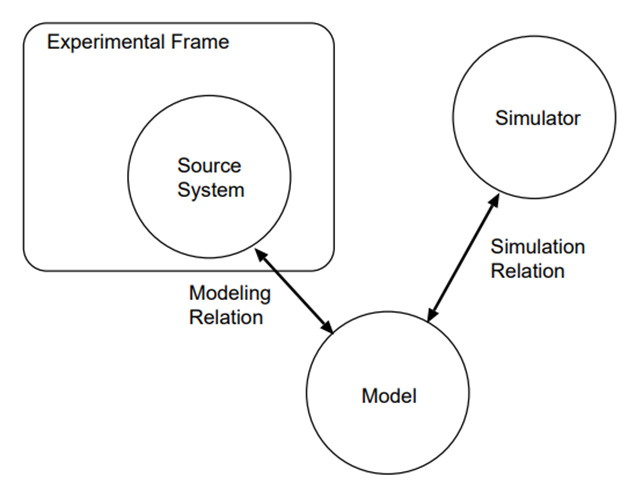
\includegraphics[width=0.7\linewidth]{images/1-modelling-and-simulation.jpg}
\caption{Basic components and relations in modeling and simulation systems\citep{FITPUB9905}}
\label{fig:figure1}
\end{figure}

\pagebreak

\noindent It is worth mentioning that \textbf{Modeling Relation} between System and Model is \textbf{isomorphic}. Isomorphic relation is commutative and for systems S1 and S2 could be written as:

$$(S1 \equiv S2) \land (S2 \equiv S1)$$

\noindent Isomorphic relation is also transitive and this condition is defined as:

$$(S1 \equiv S2) \land (S2 \equiv S3) \Rightarrow (S1 \equiv S3)$$

\vskip10pt

On the other hand, \textbf{Simulation Relation} between Model and Simulator is \textbf{homomorphic}. Homomorphic relation is simpler than the actual relation and system S1 should have more items than system S2. It is not commutative.

\vskip10pt

Simulation is organized in hierarchy. Hierarchy of Simulator is the same as hierarchy of Models. There is a root coordinator on top. Its children could be Simulators or coordinators of other Models. Parent coordinators send inputs to children, they process information and return output value with time information.

\vskip10pt

Created models need to be verified and validated. \textbf{Model verification} is a proof that Simulation Model represents abstract Model. On the contrary, \textbf{model validation} is a proof that Simulation Model represents the real system and its behavior that we are trying to reproduce and simulate.

\section{Models in DEVS}

\textbf{The atomic model} is the smallest, indivisible unit in the abstract simulation model. It is defined by the following algebraic structure \cite{DEVSformalism}:

$$M = \langle X, Y, S, S_0, t_a, \delta_{ext}, \delta_{int}, \lambda \rangle$$

\noindent where

\begin{itemize}
\item $X$ is the set of input events
\item $Y$ is the set of output events
\item $S$ is the set of sequential states
\item $s_0 \in S$ is the initial state
\item $\delta_{int} : S \to S$ is the internal transition function
\item $\delta_{ext} : Q \times X \to S$ is the external transition function, where
$$Q = \{(s,e) \mid s \in S, 0 \leq e \leq t_a(s) \}$$
describes the total state of the system at each point in time. Output $Y$ is not generated.
\item $\lambda : S \in Y \cup \{\phi\}$ is the output function. Output events are generated at the time of an internal transition. The state before the transition is used as an input to $\lambda$.
Symbol $\phi$ is considered as an unobserved event
\item $t_a : S \in T \cup \{\infty\}$ is the time advance function, which represents the time the system remains in a sequential state
\end{itemize}

\pagebreak

\noindent \textbf{The coupled model} is a network of coupled components, defined by the following algebraic structure:

$$M = \langle X, Y, D, \{M_d\}, \{I_d\}, \{Z_{i,d}\}, select \rangle$$

\noindent where

\begin{itemize}
    \item $X$ is the set of allowed external input events
    \item $Y$ is the set of allowed external output events
    \item $D$ is the set of component names
    \item $s_0 \in S$ is the initial state
    \item $M_d \mid d \in D$ is the set of components
    \item $I_d \mid d \in D \cup \{self\}$ is the set of influencees of a component
    \item $Z_{i,d} \mid i \in I_d, d \in D \cup \{self\}$ is the output-to-input translation function
\end{itemize}

\section{Ping Pong game definition in DEVS}

Firstly, I need to specify an atomic model of a Ping Pong player. It will use the same algebraic structure of atomic DEVS model:

$$PingPongPlayer = \langle X, Y, S, S_0, t_a, \delta_{ext}, \delta_{int}, \lambda \rangle$$

\noindent where

\begin{itemize}
    \item $X=\{?receive\}$
    \item $Y=\{!send\}$
    \item $S=\{Send, Wait\}$
    \item $s_0=Wait$
    \item $\delta_{int}(Send)=Wait;$ $t_a(Wait)=\infty$
    \item $\delta_{ext}(Wait, e, ?receive)=Send;$ $t_a(Send)=0.5$
    \item $\lambda(Send)=!send$
    \item $\lambda(Wait)=\phi$
\end{itemize}


\noindent I would notice that I decided to not react in any way for internal state {Wait}. Player in this state is just waiting for a ball that needs to be given to a player. Accepting a ball is processed in external transition function $\delta_{ext}(?receive)$.

\pagebreak

\noindent Definition of one single player is not enough to play a Ping Pong game. There must be exactly two players to play a game. Second player has the same structure as the first one. And it is merged with the first player into following coupled model:

$$PingPongPlayer = \langle X, Y, D, \{M_d\}, EIC, IC, EOC, select \rangle$$

\noindent where

\begin{itemize}
    \item $X=\{\}$
    \item $Y=\{\}$
    \item $D=\{Player1, Player2\}$
    \item $M_i=\{M_{player1},M_{player2}\}$ are atomic $PingPongPlayer$ models
    \item $EIC=EOC={}$
    \item $IC=\{(Player1.!send,Player2.?receive),(Player2.!send,Player1.?receive)\}$
    \item $\forall m \in 2^D-\{\} : select(m)=Player1$ for all $m \in 2^D-\{\}$
\end{itemize}

\begin{figure}[ht]
\centering
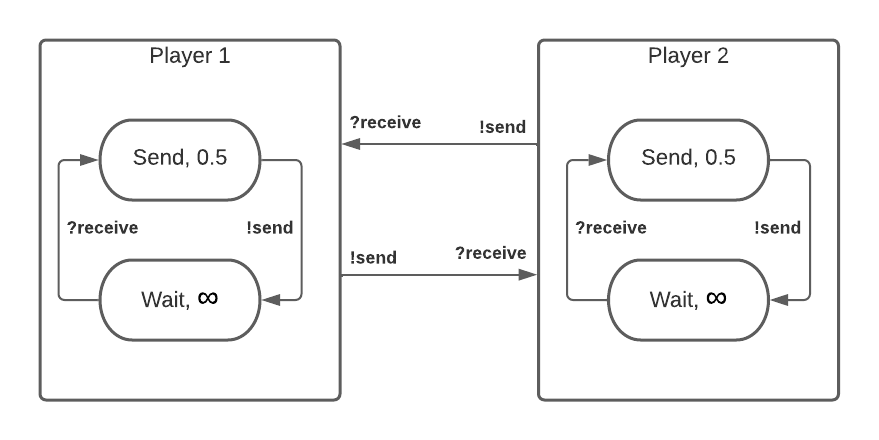
\includegraphics[width=1.0\linewidth]{images/2-CoupledDEVS - Ping Pong.png}
\caption{graphical illustration of the coupled DEVS model $PingPongGame$}
\label{fig:figure2}
\end{figure}

\section{Ping Pong game simulation in PowerDEVS}

As I mentioned at the beginning of this document, PowerDEVS is a software tool that allows atomic DEVS models to be defined in C++ language. Then we can couple them via graphical interface to a more complex model and automatically translate this model into a C++ code which executes the simulation \cite{PowerDEVS}.

\vskip10pt

All PowerDEVS source files are located at the same place where the program is installed. Important directories are:

\begin{itemize}
    \item $atomics/$ this is directory, where all atomic models are defined
    \item $examples/$ there are stored all created simulations
    \item $library/$ this directory holds definition about registered components which are able to use via graphical interface
    \item $output/$ this directory contains results of a simulation
\end{itemize}

\vskip10pt

\noindent To define a Ping Pong simulation, a new atomic model $PingPongPlayer$ must be created in the $atomics/$ folder and the atomic model definition needs to be registered in the $library/$ folder as well.

\vskip10pt

The atomic model must inherit class Simulator from PowerDEVS library $simulator.h$ and implement required methods: \textbf{init}, \textbf{ta} (the time advance function), \textbf{dint} (the internal transition function), \textbf{dext} (the external transition function), \textbf{lambda} (the output function) and exit.

\vskip10pt

Implementation of the DEVS model is pretty straightforward. To simplify code, I substitute state $\{Send\}$ and action $\{!send\}$ with value 1, which means the existence of a ball. Similarly, status $\{Wait\}$ and action $\{?receive\}$ are represented by value 0.

\vskip10pt

Infinite number is represented by an absolute value 1e20.

\vskip10pt

It is noteworthy that a player name and player speed are defined as input parameters to an atomic model, so we can set different properties for every player. It will distinguish Players between each other. One of them could be notably faster than the second one and it will bring simulation a little bit closer to a real-life game.

\vskip10pt

\lstinputlisting[caption=$PingPongPlayer$ atomic model definition in \textit{library/discrete/discrete.pdl}]{code/discrete.pdl}

\lstinputlisting[language=C++,caption=$PingPongPlayer$ atomic model definition in \textit{atomics/discrete/ping{\textunderscore}pong{\textunderscore}player.h}]{code/ping_pong_player.h}

\pagebreak

\lstinputlisting[language=C++,caption=$PingPongPlayer$ atomic model implementation defined in  \textit{atomics/discrete/ping{\textunderscore}pong{\textunderscore}player.cpp}]{code/ping_pong_player.cpp}

\pagebreak

\noindent Final $PingPongGame$ model is extended by a simple Constant output value generator. It will set an action $\{!send\}$  to Player 1 indicating that Player 1 gets a ball and starts the game.

\begin{figure}[ht]
    \centering
    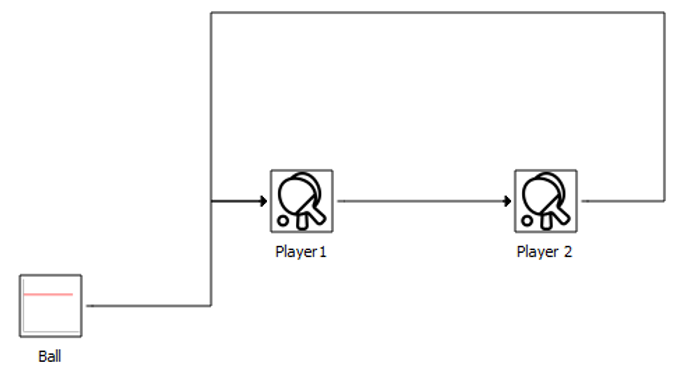
\includegraphics[width=0.8\linewidth]{images/6-ping-pong-devs.png}
    \caption{$PingPongPlayer$ model in PowerDEVS}
    \label{fig:figure4}
\end{figure}

Simulation is executed via the context window of the \textbf{Simulate button}, where final time in seconds and number of simulations could be changed. To view the results, button \textbf{View Log} opens file $output/pdevs.log$.

\begin{figure}[ht]
    \centering
    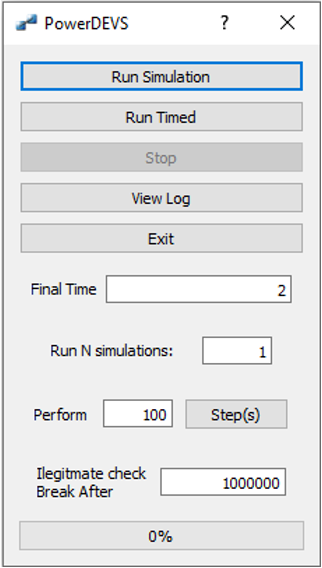
\includegraphics[width=0.35\linewidth]{images/7-simulation.png}
    \caption{"Simulate" action context window}
    \label{fig:figure5}
\end{figure}

\pagebreak

\noindent Result of example 2-seconds simulation is stated on Figure 9. As I mentioned before, I set Player reaction time via parameter speed. Player 1 speed is set to 0.51 seconds and 0.49 seconds for Player 2.

\lstinputlisting[caption=$PingPongPlayer$ simulation results in \textit{output/pdevs.log}]{code/pdevs.log}

\pagebreak

\section{Another approach – Petri Nets}

Additionally, there are also other formalisms that we could use to simulate a Ping Pong game.  Another option provides Petri Nets, which are a modeling formalism that naturally allows us to define Discrete Event Systems \cite{DeLaMotaIdaliaFlores2017RMaS}. Petri Nets is a directed, weighted and bipartite graph that is specified by:

\begin{enumerate}
    \item Place – a Ping Pong player
    \item Transition – contains pre/post conditions
    \item Directed arcs – arrows that connect transition node with place node
    \item Token – resource, in our case it is a Ping Pong ball
\end{enumerate}

PowerDEVS software tool includes Petri Nets library and thus implementation of Ping Pong game is very intuitive. Figure 10 illustrates an example simulation of a Ping Pong game in PowerDEVS tool by using Petri Nets.

\begin{figure}[ht]
    \centering
    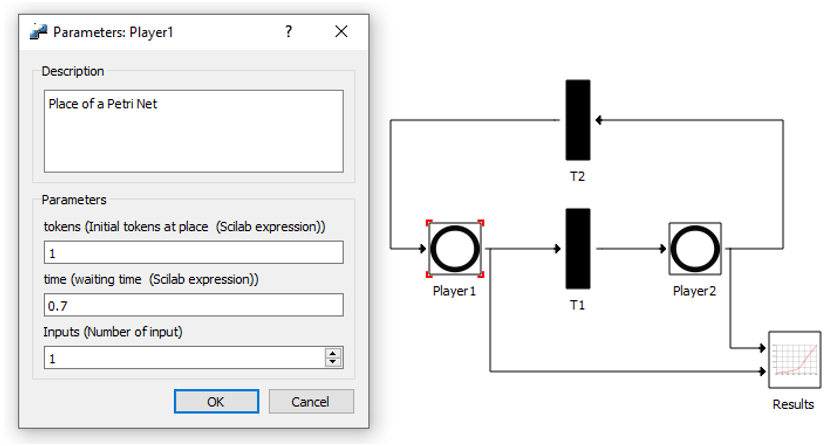
\includegraphics[width=1.0\linewidth]{images/9-ping-pong-petri.png}
    \caption{$PingPongGame$ defined by using Petri Nets}
    \label{fig:figure6}
\end{figure}

\section{Conclusion}

Firstly, I described the basics of Discrete Event System specification formalism. Secondly, I successfully defined an atomic and coupled model of a Ping Pong game in DEVS formalism. Finally, I implemented a simulation of a Ping Pong game between two players by using PowerDEVS software tool.

\vskip10pt

Since the final coupled model is discrete and time independent, I was able to execute the simulation almost immediately. This is the strongest feature of Discrete Event Systems. For instance, simulation of a 10-minutes Ping Pong game took only 1.49 seconds.


\pagebreak

\bibliography{bibliography}

\end{document}